\section{Pasos para la descarga de TIBCO EBX}

Para obtener los medios se deben seguir los siguientes pasos: 

Entrar a la página \href{https://edelivery.tibco.com/storefront/index.ep}{TIBCO EBX} y dar clic en SIGN IN. 

\begin{figure}[H]
    \centering
    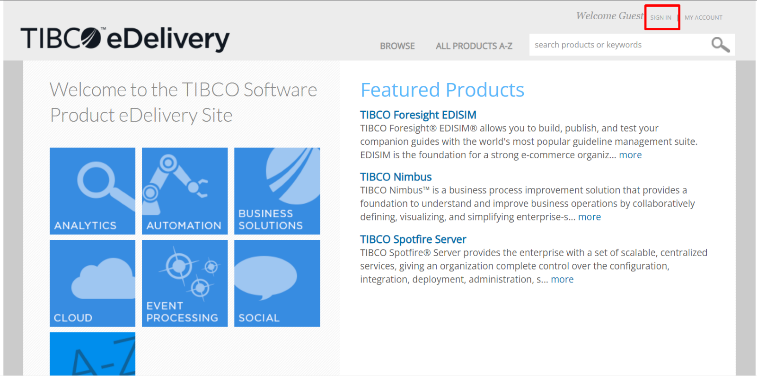
\includegraphics[width=0.4\textwidth]{Requerimientos/Instalacion/I01.png}
    \caption{Sitio oficial de descarga}
\end{figure}

Poner usuario y contraseña asignados. 
\begin{figure}[H]
    \centering
    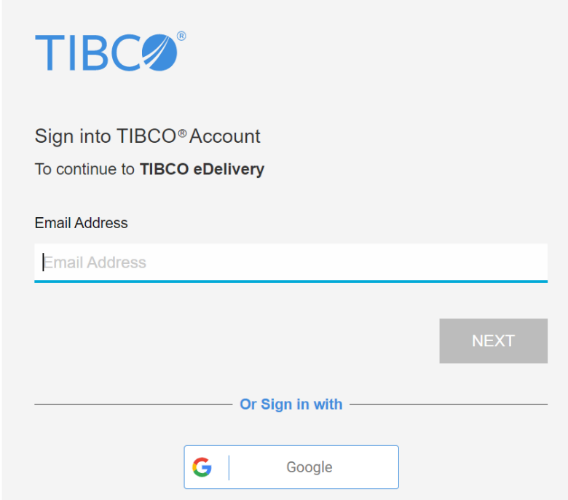
\includegraphics[width=0.4\textwidth]{Requerimientos/Instalacion/I02.png}
    \caption{Credenciales de acceso}
\end{figure}

Una vez dentro de la página, en la opción de búsqueda poner “TIBCO EBX”. 
\begin{figure}[H]
    \centering
    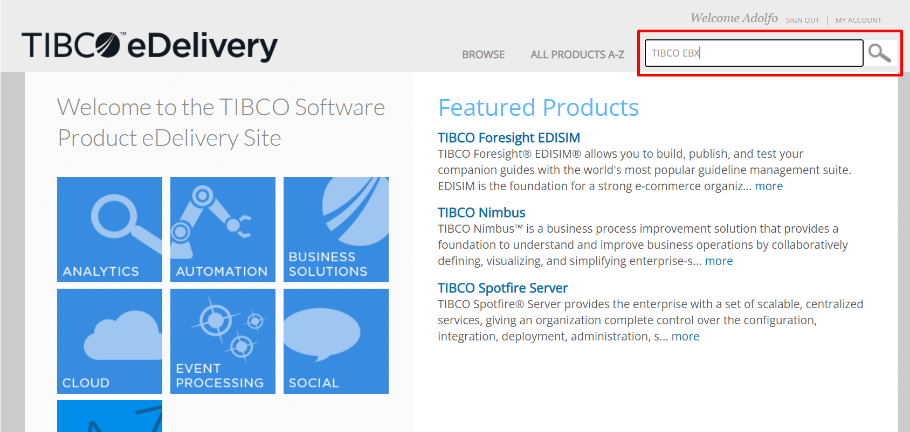
\includegraphics[width=0.4\textwidth]{Requerimientos/Instalacion/I03.png}
    \caption{Búsqueda de TIBCO EBX}
\end{figure}

Dentro de los resultados mostrados, seleccionar la opción “TIBCO EBX”. 
\begin{figure}[H]
    \centering
    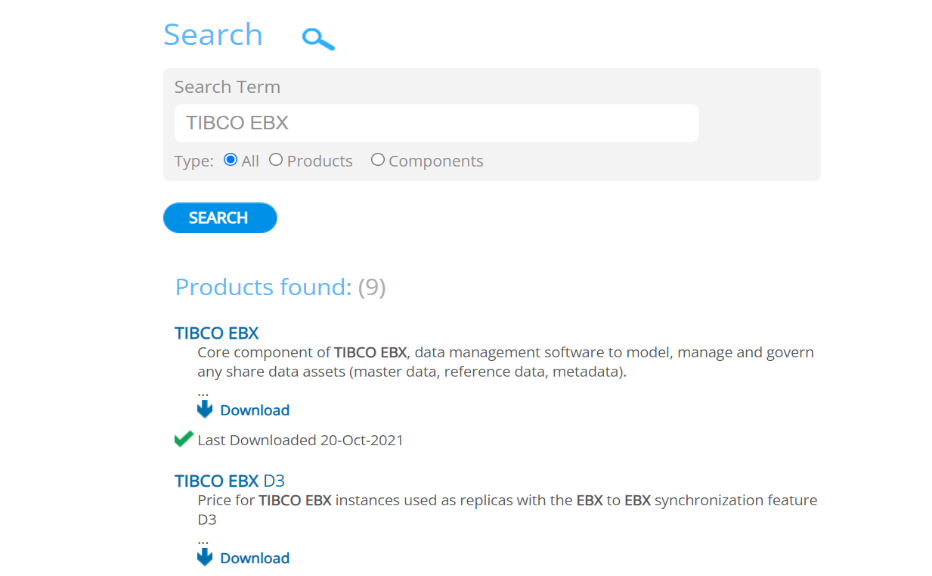
\includegraphics[width=0.4\textwidth]{Requerimientos/Instalacion/I04.png}
    \caption{Selección de TIBCO EBX}
\end{figure}

En la siguiente pantalla se dará clic en el botón “Download”. 
\begin{figure}[H]
    \centering
    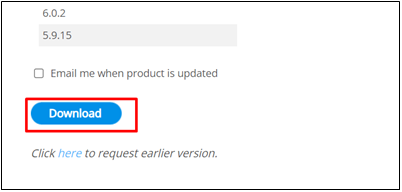
\includegraphics[width=0.4\textwidth]{Requerimientos/Instalacion/I05.png}
    \caption{Descarga de herramienta}
\end{figure}

Lo anterior redirigirá a una nueva pantalla, donde se podrá seleccionar la versión que se quiere descargar y el sistema operativo. Una vez seleccionado esto, se procede a dar clic en el botón Download: 
\begin{figure}[H]
    \centering
    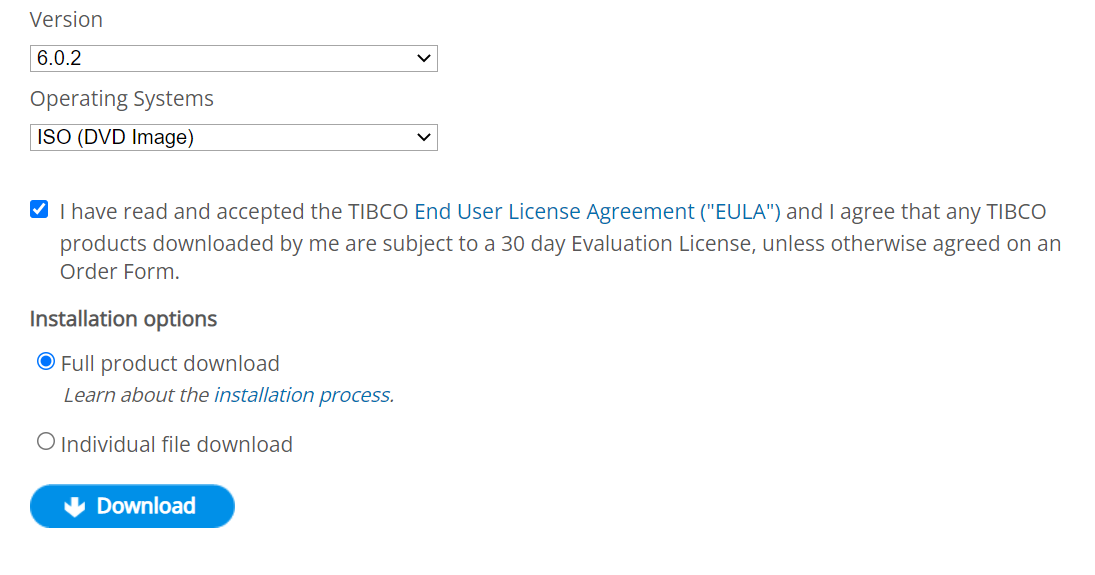
\includegraphics[width=0.4\textwidth]{Requerimientos/Instalacion/I06.png}
    \caption{Detalles de descargable}
\end{figure}

Hecho lo anterior se descargará un cliente al equipo, con el cual se puede descargar el Software. 
\begin{figure}[H]
    \centering
    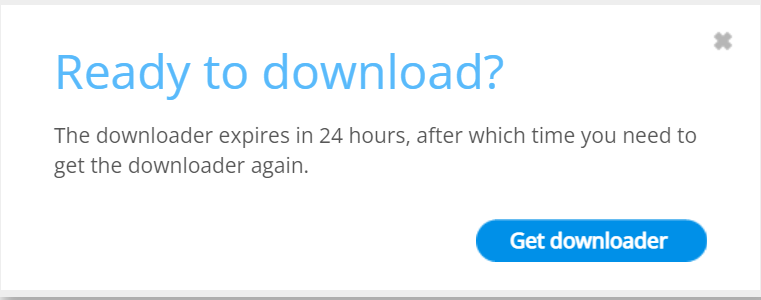
\includegraphics[width=0.4\textwidth]{Requerimientos/Instalacion/I07.png}
    \caption{Obtener Software}
\end{figure}

Se ejecuta el archivo \textbf{“Downloader - TIBCO EBX.exe”} descargado y se selecciona la ruta donde se quiere que se almacene el software, al dar clic en el botón “Next” se iniciará la descarga. 
\begin{figure}[H]
    \centering
    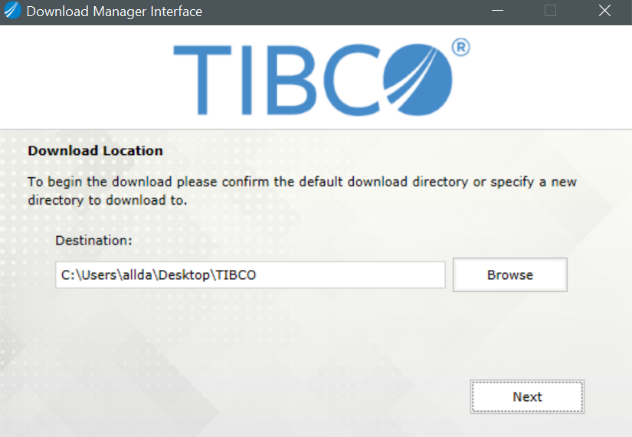
\includegraphics[width=0.4\textwidth]{Requerimientos/Instalacion/I08.png}
    \caption{Ruta de almacenamiento del Software.}
\end{figure}

Una vez que se descargue el software, éste se podrá mover al servidor y ruta deseada. 